\chapter{Einführung}

\section{Übersicht über die Applikation}
Bei dieser Applikation handelt es sich um einen
\textit{Single Player Dungeon Crawler}, der
\textit{The Binding Of Isaac} in seinen Grundzügen nachempfunden ist.
Der Spieler bewegt sich durch prozedural generierte Level. Dabei kann
er verschiedene Gegenstände einsammeln wie Rüstung (\textit{Armor}),
Waffen (\textit{Weapons}), Münzen (\textit{Coins}) und Herzen
(\textit{Hearts}). Diese Gegenstände sollen ihm dabei helfen zu
überleben. Die Münzen stellen jedoch den Punktestand dar.
Während der Spieler sich durch die Räume bewegt, stößt er
auf eine Palette unterschiedlicher Gegner (\textit{Spider}, 
\textit{Skeleton}, {Zombie}, \textit{Ogre}). Diese besitzen auch
unterschiedliche Fähigkeiten und versuchen den Spieler zu besiegen.
Betritt der Spieler einen Raum, so wird dieser gesperrt, bis er alle
darin befindlichen Gegner besiegt hat. Erst dann öffnen sich die Türen
wieder und der Spieler kann in anliegende Räume laufen.
Stirbt der Spieler dabei, so ist das Spiel zu Ende. Bleibt er am Leben,
hangelt er sich von Level zu Level. Am Ende eines jeden Levels steht
ein Raum mit einer einzigen Falltür in der Mitte, welche den Spieler
in das nächste Level bringt.

Das Spiel ist rundenbasiert. In jeder Runde stehen Aktionen zur 
Verfügung, wie etwa Angreifen (\textit{Space}), Bewegen
(\textit{W}, \textit{A}, \textit{S} oder \textit{D}) oder Aufheben
(\textit{E}). Auch die Gegner agieren rundenbasiert. Diese können
jedoch lediglich angreifen. Sie laufen dem Spieler mit einer Runde
Zeitversatz hinterher. Dabei können Gegner sich auch gegenseitig den
Weg blockieren.

Damit der Spielstand in Form von Level, Gegnern und Items nachvollziehbar
bleibt, gibt es eine einfache Anzeige, welche mithilfe von ANSI- und
ASCII-Zeichen den Spielinhalt darstellt. Dabei helfen unterschiedliche
Symbole und Farben den Inhalt zu verstehen.

\section{Wie startet man die Applikation?}
Voraussetzung ist \textbf{Java 19}. Optimalerweise wird das Programm
in einem ANSI-fähigen Terminal (Farbunterstützung und Kontrollzeichen)
gestartet. Diese werden bei den allermeisten Linux Distributionen
(z.B. Ubuntu) direkt mitgeliefert. Alternativ funktioniert auch die
IntelliJ-Konsole. \newline

\textbf{Ausführung in Konsole}:

Bei Vorliegen der JAR-Datei folgenden Befehl ausführen: \newline
\texttt{/home/<User>/.jdks/openjdk-19.0.2/bin/java -jar ASE.jar} \newline

\textbf{Ausführung in IntelliJ}:

Im Projekt befindet sich unter \texttt{./src/main/java/plugins}
die Klasse \textit{Main} mit der obligatorischen \textit{main()}-Methode.
Diese Methode lässt sich mittels Knopfdruck ausführen. \newline

\textbf{Anmerkung}:

Um externe Abhängigkeiten zu minimieren, wurde auf eine
Key-Input-Library verzichtet. Für die Interaktion benötigen wir
allerdings spontane Tasteneingaben, welche nicht durch \textit{Enter}
bestätigt werden. Die Lösung in Java ist daher, ein winziges Fenster
mit Fokus zu öffnen. Auf diesem ist ein \textit{KeyListener} registriert,
welcher die spontanen Tasteneingaben entgegennimmt und an das eigentliche
Programm weiterleitet. Damit erhält man auch in der Konsole direkte
Interaktivität.

Der Nachteil ist allerdings, dass der Fokus auf dieses Fenster für einen
normalen Benutzer nur schwierig wieder zu erlangen ist, sobald eine
Maus-Interaktion außerhalb des Programmes getätigt wurde. Dann wird
nämlich der Fokus durch das Betriebssystem vom Fenster genommen.

Daher ist darauf zu achten, dass, sobald das Programm gestartet ist,
lediglich Tasteneingaben erfolgen. Ansonsten muss das Programm
neu gestartet werden, damit das Fenster wieder den Fokus hat. Die
Applikation kann in der Konsole dennoch mittels der Tastenkombination
\textit{Ctrl + C} mit einem Signal beendet werden.

Im Übrigen sollte das Konsolen-Interface wie folgt aussehen. Sind
unpassende Zeichen zu sehen oder fehlen Farben, dann ist das Terminal
nicht im richtigen Modus oder unterstützt grundsätzlich nicht die
Darstellung. Ein Unix-Terminal oder die IntelliJ-Konsole schaffen 
dabei Abhilfe.

\vspace{0.5cm}
\begin{figure}[H]
    \centering
    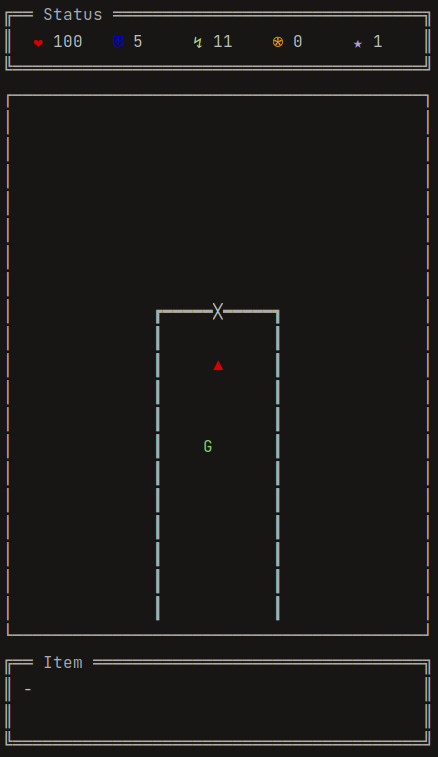
\includegraphics[width=0.6\linewidth]{Bilder/Visualisierung/GameLook.png}
    \caption{Konsolen-Interface}
\end{figure}

\section{Wie testet man die Applikation?}
